
\chapter{\'Etudes de cas et exp\'erimentations~: Comparaisons de \ppff\ avec Java et FastFlow}
\label{experiences.chap}

\gt{Pas besoin de dire que c'est <<possibilit\'es d'utilisation>>. Tu
as d\'evelopp\'e une bibloth\`eque, et tu veux voir comment elle se
compare avec d'autres.}

Ce chapitre pr\'esente une \'evaluation exp\'erimentale de \TT{PpFf} afin de comparer ses performances avec d'autres approches d'ex\'ecution parall\`ele, plus sp\'ecifiquement avec \TT{Java} et \TT{FastFlow}.
%
Dans les sections~\ref{wordcount.sect} et~\ref{stockprice.sect}, nous pr\'esentons deux applications \'ecrites avec \PpFf. Ces applications ont \'et\'e choisies non seulement pour montrer certaines fonctionnalit\'es de l'API, mais \'egalement pour leur pertinence dans des sc\'enarios typiques. La section~\ref{wordcount.sect} pr\'esente une application permettant de calculer le nombre d'occurrences des mots dans un texte --- le <<\emph{Hello World!}>> des syst\`emes de traitement de donn\'ees en mode \emph{batch} --- alors que la section~\ref{stockprice.sect} pr\'esente une application permettant de calculer des statistiques sur les prix d'indices boursiers --- un exemple typique de traitement de flux en ligne (\emph{online data processing}). La derni\`ere section, la section~\ref{coutsPpFf.sect}, pr\'esente une application permettant de d\'eterminer les surco\^uts introduits par \TT{PpFf} par rapport \`a \TT{FastFlow} --- un \emph{micro benchmark} consistant en un pipeline avec un seul op\'erateur.
%
\GT{Il faut aussi mentionner la section~\ref{coutsPpFf.sect}.}
\IC{J'ai mentionn\'e la derni\`ere section.}
%
Mais tout d'abord, nous pr\'esentons la fa\c{c}on dont nos
exp\'erimentations ont \'et\'e effectu\'ees.

\section{M\'ethode utilis\'ee pour les exp\'erimentations}
\label{usedMethodsForBenchmarks.chap}

Chaque syst\`eme informatique a des caract\'eristiques propres. Les principaux facteurs qui influencent les performances d'un tel syst\`eme sont le type de processeur, le nombre de processeurs ou de c\oe{}urs, et le r\'eseau de communication. 


\gt{Ne sp\'ecifie pas que tu as utilis\'e un nombre fixe de machines,
parce que si des scripts gnuplots sont d\'efinis \`a un moment, je
pourrais essayer de rouler les benchmarks aussi sur une de mes
machines --- il me semble que sur ma machine Linux, les r\'esultats
\'etaient mieux qu'ailleurs, non? Je ne suis plus certain!?}


\gt{Une fa\c{c}on possible pour \'eviter l'ambiguit\'e machine Java
vs.\ langage Java~: introduire un identificateur pour la machine, et
ensuite utiliser cet identificateur dans les diagrammes?}


\goodbreak
\begin{samepage}
Afin d'avoir des r\'esultats plus g\'en\'eraux, nous avons conduit nos exp\'eriences sur les machines suivantes~:
\label{machines.sect}

\gt{J'ai introduit une macro M/Machine,  pour que la forme soit
toujours la m\^eme partout.}

\ic{Tr\`es utile.}

\begin{description}
\item[\M1] = \TT{java.labunix.uqam.ca}~: Une machine avec 16 processeurs de 2,6 GHz, chacun contenant 6 cœurs. Le syst\`eme d'exploitation est Linux version 3.10.0. 


\item[\M2] = \TT{japet.labunix.uqam.ca}~:  Une machine avec 64 processeurs de 2,3 GHz, chacun contenant 8 cœurs. Le système d'exploitation est Linux version 3.10.0.

\gt{Vraiment? Donc 512 coeurs en tout? Cela m'\'etonne!}

\end{description}
\end{samepage}

% GT: Je ne comprends pas le role de cette phrase. Je l'ai supprimee.
%Dans un environnement de traitement de flux, les donn\'ees sont g\'en\'eralement transform\'ees au fur et \`a mesure de leur progression dans le pipeline. 

\gt{Ci-bas: est-ce ok comment j'ai modifi\'e?}

\ic{Beaucoup mieux. J'ai chang\'e seulement le nombre de r\'ep\'etition. J'ai chang\'e 20 pour 10.}

Chaque exp\'erience --- i.e., un lancement d'un programme --- a \'et\'e ex\'ecut\'ee plusieurs fois pour obtenir un r\'esultat stable, puisque le temps d'ex\'ecution peut varier beaucoup d'une ex\'ecution \`a une autre. 
%Le nombre de r\'ep\'etitions de chaque exp\'erience a \'et\'e vari\'e, puis nous avons pris le facteur de r\'ep\'etitions pour les meilleurs r\'esultats obtenus.
%
Pour les r\'esultats pr\'esent\'es dans les sections suivantes, le nombre de r\'ep\'etitions a \'et\'e \'etabli \`a~10; le temps d'ex\'ecution de r\'ef\'erence pour une exp\'erience est donc la \emph{moyenne} des temps de 10 ex\'ecutions.


\gt{Ici, il faut donner une vue d'ensemble de la fa\c{c}on dont tu as
proc\'ed\'e~: quelles machines (architecture, OS, etc. Parler comme tu
fais ci-bas que chaque {\bf programme \emph{benchmark}} est ex\'ecut\'e
plusieurs fois, comment ce temps est mesur\'e (de l'int\'erieur du
programme par des appels syst\`emes internes), que la moyenne des
temps d'ex\'ecution est calcul\'ee pour obtenir un r\'esultat plus
juste/stable, etc.}

\gt{Ensuite, tu pourras d\'ecrire les r\'esultats pour chacun des
programmes.}

\ic{J'ai d\'ecrit un peu comment j'ai ex\'ecut\'e les tests.}


\gt{Ce n'est pas encore clair pour moi.  Tu as lanc\'e le m\^eme
programme 20 fois, puis tu as calcul\'e la moyenne des 20 r\'esultats
obtenus?  Ou bien chaque programme est ex\'ecut\'e une fois, mais en
roulant son corps 20 fois?  Habituellement, c'est la premi\`ere
approche qu'on utilise, parce qu'un lancement d'un programme varie
d'une fois \`a une autre, selon la charge de la machine, du r\'eseau,
etc. Donc, on lance le programme $NB$ fois (par ex., NB=10), on mesure
le temps pour chaque ex\'ecution et on fait la moyenne des $NB$
temps.}



Il faut noter que le fonctionnement des programmes \TT{Java} et~\TT{PpFf} n'est pas le m\^eme. Alors que \TT{PpFf} permet de varier le nombre de fils d'ex\'ecution (\emph{threads}), \TT{Java} ne le permet pas. Afin de montrer les meilleurs temps d'ex\'ecution et l'\'evolutivit\'e de \TT{PpFf}, plusieurs exp\'eriences ont \'et\'e men\'ees en variant le nombre de \emph{threads}. Par contre, dans le cas de \TT{Java}, pour chaque exp\'erience, deux s\'eries de tests ont \'et\'e ex\'ecut\'ees: une s\'erie avec le \emph{JIT} (\emph{Just-In-Time compiler}) et l'autre sans.

\label{jitDescription.sect}
\emph{JIT}~\citep{cramer1997compiling} est un composant de l'environnement d'ex\'ecution Java qui am\'eliore les performances des applications en compilant le \emph{bytecode} de la machine virtuelle en code machine \emph{au moment de l'ex\'ecution}. Le \emph{bytecode} est l'ensemble des instructions de la \emph{JVM} (\emph{Java Virtual Machine}) qui permet aux applications d'\^etre ex\'ecut\'ees sur plusieurs plates-formes. Comme on le verra, la conversion du \emph{bytecode} en langage machine a un impact significatif sur la vitesse d'ex\'ecution.

\gt{Je crois qu'il faut aussi que tu parles du JIT, que tu vas
comparer l'ex\'ecution du programme Java avec le JIT activ\'e vs.\
sans le JIT. Tu pourrais alors r\'ef\'erer, par exmple, \`a la machine
\M{1+} avec JIT et \M{1-} sans JIT.}

\ic{Ici plus haut, j'ai parl\'e de JIT.}


\section{\emph{Word Count}}
\label{wordcount.sect}

\gt{En anglais, c'est <<appendix>> mais en fran\c{c}ais c'est annexe!}

\gt{Je crois qu'il serait pr\'ef\'erable de pr\'esenter les mesures
associ\'ees dans la m\^eme section, sinon ta section 4.2 sera courte
et ce sera m\'elangeant d'avoir les r\'esultats \`a part.}

\gt{Donc, 4.2 (idem pour 4.3) pourrait contenir: 4.2.1 Description de
l'application; 4.2.2 Mesures obtenues; 4.2.3 Analyse des r\'esultats.}

\ic{Bonne id\'ee}


\subsection{Description de l'application \TT{Stock Price}}

\GT{J'ai chang\'e <<Stock Market>> pour <<Stock Price>> car c'est ce
que tu semblais utiliser dans le code et \`a plusieurs endroits.}

\IC{C'est vrai. Je n'ai pas accord\'e attention \`a la diff\'erence entre les deux titres.}

Dans la section.~\ref{descriptionWordCount.sect}, nous avons pr\'esent\'e \TT{WordCount}, une application simple qui compte le nombre d'occurrences des divers mots dans un fichier texte. L'application prend en entr\'ee un fichier texte et produit un conteneur de type \TT{map<string, int>} où la cl\'e repr\'esente un mot dans le fichier et la valeur  type \TT{int}  associ\'ee repr\'esente le nombre d'occurrences du mot dans le fichier. Le code source des applications \TT{WordCount} en~\TT{PpFf} et~\TT{Java} est pr\'esent\'e dans les annexes~\ref{sourceCodeWordCountPpFf.ann} et~\ref{sourceCodeWordCountJava.ann} respectivement.


\subsection{Mesures obtenues et analyse des r\'esultats}


%Plots bar examples: http://pgfplots.net/tikz/examples/tag/bar-plots/


%
%\begin{tikzpicture}
%\begin{axis}[
%    title={WordCount - machine Java; sans JIT; 1 itération; PpFf-1 thread\bigskip},
%    xlabel={Nb.~mots},
%    ylabel={Temps d'ex\'ecution (ms)},
%    xmin=0, xmax=5500000,
%    ymin=0, ymax=25000,
%    ytick={0,5000,10000,15000,20000,25000},
%    %xtick={0,500000,1000000,1500000,3000000,4500000,5000000,5500000},
%    xtick={0,1000000,2000000,3000000,4000000,5000000,6000000},
%    legend pos=north west,
%    ymajorgrids=true,
%    grid style=dashed,
%]
% 
%\addplot[
%    color=blue,
%    mark=square,
%    ]
%    coordinates {
%    (78792,106)(67941,205)(281307,322)(482636,508)(752856,883)(2614743,3320)(5247678,6126)
%    };
%\addplot[
%    color=red,
%    mark=square,
%    ]
%    coordinates {
%    (78792,1615)(167941,2319)(281307,3625)(482636,4906)(752856,7195)(2614743,116039)(5247678,226917)
%    };
%\legend{PpFf,Java}    
%\end{axis}
%\end{tikzpicture}


%
%\begin{figure}[H]
%\centering
%	\begin{tikzpicture}
%	\begin{axis}[
%	    xlabel={Nb.~mots},
%    	ylabel={Temps d'ex\'ecution (ms)},
%	    xmin=0, xmax=5500000,
%    	ymin=0, ymax=5500,
%	    %ytick={0,500,1000,1500,2000,2500,3000,3500,4000,4500,5000,5500},
%    	ytick={0,1000,2000,3000,4000,5000,6000},
%	    xtick={0,1000000,2000000,3000000,4000000,5000000,6000000},
%    	legend pos=north west,
%	    ymajorgrids=true,
%    	grid style=dashed,
%	]
% 
%	\addplot[
%    	color=blue,
%   	 	mark=square,
%    ]
%    	coordinates {
%    	(78792,174)(67941,117)(281307,263)(482636,405)(752856,429)(2614743,1625)(5247678,2798)
%    	};
%	\addplot[
%    	color=red,
%    	mark=square,
%    ]
%    	coordinates {
%    	(78792,368)(167941,443)(281307,501)(482636,603)(752856,730)(2614743,3889)(5247678,5312)
%    	};
%	\legend{PpFf,Java}    
%	\end{axis}
%	\end{tikzpicture}
%    \caption{Les temps d'ex\'ecution pour \TT{WordCount} sur la machine Japet.}
%    \label{JapetExecutionWordCount.fig}	
%\end{figure}


\begin{figure}
\centering
     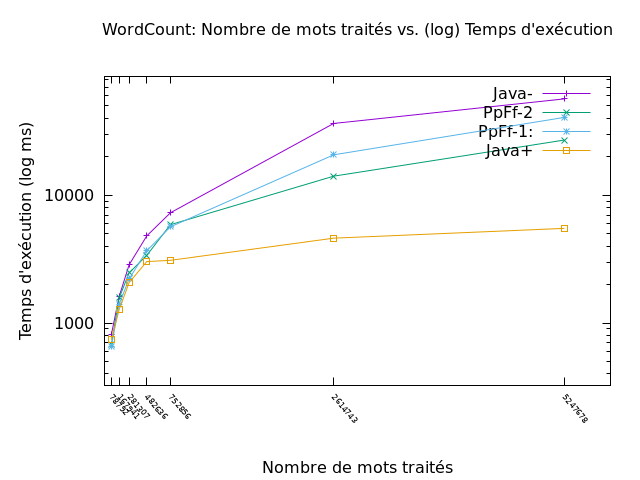
\includegraphics[width=1.0\textwidth]{Figures/graphe_temps_Java_WordCount.png}
      \caption{Les temps d'ex\'ecution pour \TT{WordCount} sur la machine \M1.}
       \label{GrapheTempsWordCountJava.fig}
\end{figure}

\begin{figure}
\centering
     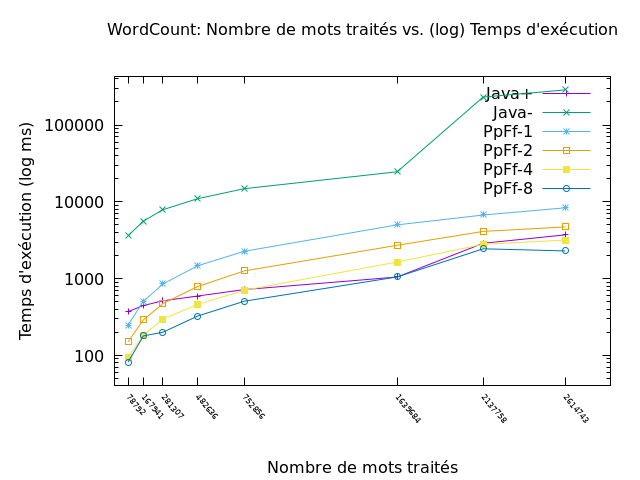
\includegraphics[width=1.0\textwidth]{Figures/graphe_temps_Japet_WordCount.png}
      \caption{Les temps d'ex\'ecution pour \TT{WordCount} sur la machine \M2.}
       \label{GrapheTempsWordCountJapet.fig}
\end{figure}

\gt{Ci-bas: ultimement, il faudra pr\'esenter dans le texte dans le
m\^eme ordre que les num\'eros, donc 4.1 avant 4.2!}

\ic{J'ai r\'evis\'e l'analyse selon les nouveaux r\'esultats des exp\'eriences.}

Dans cette section, nous 
% présentons une \'evaluation exp\'erimentale approfondie pour les op\'erations d\'ecrites dans la section pr\'ec\'edente. Nous
\'evaluons l'application \TT{WordCount} en examinant le temps d'ex\'ecution requis en fonction du nombre de mots. Afin de conna\^itre l'impact de la quantit\'e de donn\'ees \`a traiter, les exp\'eriences ont \'et\'e men\'ees en utilisant plusieurs ensembles de donn\'ees. Chaque ensemble de donn\'ees --- un fichier sur disque --- contient un nombre croissant de mots. Ces nombres de mots varient de 78~792 \`a 2~614~743. Pour toutes les exp\'eriences, le facteur de r\'ep\'etitions a \'et\'e \'etabli \`a 10.  Les r\'esultats sont pr\'esent\'es dans les figures~\ref{GrapheTempsWordCountJava.fig} et~\ref{GrapheTempsWordCountJapet.fig} respectivement: la figure~\ref{GrapheTempsWordCountJava.fig} montre les résultats obtenus sur la machine \M1\ alors que la figure~\ref{GrapheTempsWordCountJapet.fig} montre ceux obtenus sur la machine M2. Repr\'esent\'es sur les deux axes des diagrammes, les r\'esultats sont interpr\'et\'es \`a l'aide des deux m\'etriques : le nombre de mots sur l'axe x et le temps d'ex\'ecution sur l'axe y.  Afin de visualiser l'ensemble des exp\'eriences sur une m\^eme figure, l'\'echelle pour le temps d'ex\'ecution est logarithmique. 

Deux s\'eries d'exp\'eriences ont \'et\'e men\'ees dans le cas de \TT{Java}. L'une avec \emph{JIT} et l'autre sans. Les r\'esultats de ces exp\'eriences sont marqu\'es dans les deux diagrammes par \TT{Java+} et \TT{Java-} respectivement. Dans le cas de \TT{PpFf}, les exp\'eriences ont \'et\'e men\'ees en variant les nombres de \emph{threads}. Deux \emph{threads} ont \'et\'e utilis\'es sur la machine \M1\ et huit sur la machine \M2. Le suffixe de type int\`egre dans les notations de \TT{PpFf} de deux diagrammes repr\'esente le nombre de \emph{threads} utilis\'es dans les exp\'eriences. Par exemple dans la notation \TT{PpFf-2}, deux \emph{threads} ont \'et\'e utilis\'es et dans la notation \TT{PpFf-4}, quatre \emph{threads} ont \'et\'e utilis\'es.


\GT{Il faut expliquer un peu plus ces figures, notamment: i) le fait
que l'\'echelle pour le temps d'ex\'ecution est logarithmique (pour
permettre de voir l'ensemble des exp\'eriences sur une m\^eme
figure. ii) expliquer bri\`evement les \'etiquettes utilis\'ees~:
Java- vs. Java+, PpFf-*}

\IC{J'ai ajout\'e des explications suppl\'ementaires.}

Les exp\'eriences men\'ees sur la machine \M1\ montrent que le temps d'ex\'ecution de \TT{Java} sans \TT{JIT} est nettement sup\'erieur \`a celui avec \TT{JIT}. Dans le cas de \TT{PpFf}, le temps d'ex\'ecution avec un \emph{thread} par rapport \`a celui avec deux \emph{threads} est meilleur lorsque la charge du travail est petite. Cela peut s'expliquer par les surco\^uts suppl\'ementaires introduits par la cr\'eation de \emph{threads}.

En comparant les temps d'ex\'ecutions entre \TT{PpFf} et \TT{Java}, on constate que, pour une petite charge de travail, \TT{PpFf} obtient de meilleurs temps d'ex\'ecution. Lorsque la charge du travail augmente, \TT{Java} se comporte mieux. Cela peut \^etre observ\'e dans la figure~\ref{GrapheTempsWordCountJava.fig}, o\`u \TT{Java} obtient de meilleurs temps d'ex\'ecution par rapport \`a \TT{PpFf--1}. 

La gestion de \emph{threads} entre les deux programmes diff\`ere. \TT{PpFf} ex\'ecute chaque op\'eration d'un \TT{pipeline} sur un \emph{thread} diff\'erent. Par exemple, les cinq op\'erations de \TT{WordCount} --- \TT{source}, \TT{flatMap}, \TT{map}, \TT{find} et \TT{reduceByKey} --- s'ex\'ecutent sur cinq \emph{threads} diff\'erents. Par contre, \TT{Java} g\`ere la cr\'eation de \emph{threads} par l'interm\'ediaire du \emph{framework} \TT{fork/join}. D\'ecrit dans le chapitre~\ref{outils_connus.chap} (p.~\pageref{forkjoin.sect}), le \emph{framework} divise une t\^ache en plus petites sous-t\^aches ind\'ependantes, et ce r\'ecursivement jusqu'\`a ce qu'elles soient assez simples pour \^etre ex\'ecut\'ees. Ce m\'ecanisme permet \`a \TT{Java} d'\^etre plus efficace que \TT{PpFf--1}. \TT{PpFf} est plus rapide que \TT{Java} lorsqu'on augmente le nombre de \emph{threads}. On peut observer cela dans la figure~\ref{GrapheTempsWordCountJava.fig}. \TT{PpFf--2} obtient de meilleurs temps d'ex\'ecution que \TT{Java} pour une charge de travail plus grande.

Les m\^emes exp\'eriences ont \'et\'e men\'ees sur la machine \M2. Par rapport \`a la machine \M1\, \M2\ dispose de plusieurs processeurs. Cela nous a permis d'ex\'ecuter plusieurs s\'eries d'exp\'eriences en faisant varier le nombre de \emph{threads} dans le programme \TT{PpFf}. La figure~\ref{GrapheTempsWordCountJapet.fig} montre les r\'esultats obtenus pour les deux programmes. On peut constater que \TT{PpFf} obtient de meilleurs temps d'ex\'ecution  que \TT{Java}. 


\GT{Surtout pour \M2, ce serait bien de voir/discuter si
l'augmentation du temps d'ex\'ecution augmente de fa\c{c}on lin\'eaire
avec l'augmentation du nombre de mots trait\'es?}

\IC{Je ne sais pas exactement de ce que je dois parler. Est-ce que je dois parler d'une seule s\'erie d'exp\'eriences? Par exemple, en prenant PpFf-8, je d\'etermine le nombre de mots trait\'e par ms pour chaque fichier et ensuite je d\'etermine si ce r\'esultat est lin\'eaire. Je ne sais pas ce que je dois montrer avec ce r\'esultat. Ou je dois arriver ? }

\section{\emph{Stock Price}}
\label{stockprice.sect}

\gt{En anglais <<stock>> est, en fran\c{c}ais, une <<action (boursi\`ere)>>.}

Dans le monde informatique actuel, les institutions financi\`eres produisent d'\'enormes quantit\'es d'informations, par ex., des informations sur les march\'es boursiers. Un probl\`eme important qu'elles rencontrent consiste \`a trouver des moyens efficaces pour r\'esumer et visualiser les donn\'ees afin de produire des informations utiles sur le comportement du march\'e, notamment pour prendre des d\'ecisions d'investissement. Cette section pr\'esente une application qui calcule le prix maximum pour diverses actions d'un marché boursier. Le code source des applications \TT{StockPrice} en \TT{PpFf} et~\TT{Java} sont pr\'esent\'es dans les annexes~\ref{sourceCodeStockPricePpFf.ann} et~\ref{sourceCodeStockPriceJava.ann} respectivement. 

\subsection{Description de l'application}

L'application \TT{Stock Price} calcule le prix d'une action en utilisant le modèle \emph{Black-Scholes}~\citep{macbeth1979empirical}. Ce mod\`ele d'\'evaluation est utilis\'e pour d\'eterminer le prix juste ou la valeur th\'eorique d'une option d'achat ou de vente, et ce en fonction de six variables telles que la valeur de l'action sous-jacente, le prix d'exercice, le taux d'int\'er\^et sans risque, la volatilit\'e du prix de l'action, la dur\'ee et le type d'option. 

L'application \TT{Stock Price} est compos\'ee de cinq op\'erations principales~: 

\begin{lstlisting}[
label={exampleInfoActionFromFile},
language=c++,
caption={Un exemple illustrant l'information sur des actions contenues dans le fichier.},
frame=single,
float]
SNY 100.00 90.00 0.1000 0.00 0.10 1.00 C 0.00 18.6308591206674982
JCI 100.00 100.00 0.1000 0.00 0.10 0.50 C 0.00 5.8502736042849798
DSX 100.00 100.00 0.1000 0.00 0.10 1.00 C 0.00 10.3081472436668
LILA 100.00 110.00 0.1000 0.00 0.10 0.10 C 0.00 0.003523074865
NVS 100.00 110.00 0.1000 0.00 0.10 0.50 C 0.00 1.1407228438274099
FLML 100.00 110.00 0.1000 0.00 0.10 1.00 C 0.00 4.216747020308
TEF 100.00 90.00 0.1000 0.00 0.25 0.10 C 0.00 11.1352446183467002
DXB 100.00 90.00 0.1000 0.00 0.25 0.50 C 0.00 16.0926388440922991
HSEA 100.00 90.00 0.1000 0.00 0.25 1.00 C 0.00 21.16345465848
LENS 100.00 100.00 0.1000 0.00 0.25 0.10 C 0.00 3.65996266031
\end{lstlisting}

\begin{itemize}

\item Une op\'eration qui d\'efinit la source du flux de donn\'ees. Ici, la source est constitu\'ee par les lignes contenues dans un fichier. Le listing~\ref{exampleInfoActionFromFile} montre un exemple avec quelques enregistrements tir\'es de notre fichier de test. 

Un enregistrement est identifi\'e par les informations suivantes : le nom de l'action, la valeur actuelle de l'action sous-jacente, le prix d'exercice, le taux d'int\'er\^et sans risque, le taux de dividende, la volatilit\'e du prix de l'action, le temps qu'il reste \`a l'option avant son \'ech\'eance (exprim\'e en ann\'ees), le type d'option (\TT{C=CALL}~: prix pour une option d'achat~; \TT{P=PUT}~: prix pour une option de vente), la valeur de dividende et la valeur de r\'ef\'erence \TT{DerivaGem}. 
Les valeurs \TT{DerivaGem}, la valeur et le taux de dividende ne sont pas utilis\'es dans \TT{Stock Price} pour calculer le prix d'une action.

\item Une op\'eration qui r\'epartit les \'el\'ements du flux entre divers \emph{threads}.
Toutes les \'etapes qui suivent cette op\'eration seront donc ex\'ecut\'ees en parall\`ele.

\item Une op\'eration  \TT{map}, qui permet d'extraire le nom et les options de chaque action.

\gt{En fait, que contient un enregistrement: les infos sur une action
sp\'ecifique? Ou une transaction boursi\`ere? \`A clarifier!}

\ic{Bonne question. J'imagine qu'il s'agit d'actions enregistr\'ees \`a la suite de transaction boursi\`ere. J'ai regard\'e la description de Pico. Il n'y a pas beaucoup de d\'etails. https://github.com/alpha\-unito/pico/tree/master/examples/stock-market. (The stock\_pricing.cpp code is an example of batch pipeline (like word\-count), meaning file\-based I\/O. It takes in input a series of stock records and computes the maximum price for each stock name.) }

\item  Une op\'eration qui calcule le prix de chaque action. L'algorithme utilis\'e est celui de \emph{Black-Scholes}~\citep{macbeth1979empirical}. 

\item Une derni\`ere op\'eration qui extrait le prix maximum pour chaque action.


\end{itemize}

\subsection{Mesures obtenues et analyse des r\'esultats}

%
%\pgfplotstableread[row sep=\\,col sep=&]{
%    interval & PpFf & Java \\
%    M1+  & 302 & 574 \\
%    M1-   & 504 & 2696 \\
%    M2+   & 357 & 402 \\
%    M2-   & 350 & 5810 \\
%    }\mydata
%
%
%\begin{figure}[H]
%\centering
%	\begin{tikzpicture}
%    	\begin{axis}[
%            ybar,
%            bar width=.5cm,
%            width=.7\textwidth,
%            height=.5\textwidth,
%            legend style={at={(0.5,1)},
%                anchor=north,legend columns=-1},
%            symbolic x coords={M1+, M1-, M2+, M2-},
%            xtick=data,
%            nodes near coords,
%            nodes near coords align={vertical},
%            ymin=0,ymax=6000,
%            ylabel={Temps d'ex\'ecution (ms)},
%        ]
%        \addplot table[x=interval,y=PpFf]{\mydata};
%        \addplot table[x=interval,y=Java]{\mydata};
%        \legend{PpFf, Java}
%    	\end{axis}
%	\end{tikzpicture}
%    \caption{Les temps d'ex\'ecution pour l'application \TT{Stock Price}.}
%    \label{executionTimesStockPrice.fig}
%\end{figure}


\pgfplotstableread[row sep=\\,col sep=&]{
    interval & PpFf & Java \\
    M1  & 232 & 1629 \\
    M2  & 304 & 411 \\
    }\mydata


\begin{figure}[H]
\centering
	\begin{tikzpicture}
    	\begin{axis}[
            ybar,
            bar width=.5cm,
            width=.7\textwidth,
            height=.5\textwidth,
            legend style={at={(0.5,1)},
                anchor=north,legend columns=-1},
            symbolic x coords={M1, M2},
            xtick=data,
            nodes near coords,
            nodes near coords align={vertical},
            ymin=0,ymax=2000,
            ylabel={Temps d'ex\'ecution (ms)},
        ]
        \addplot table[x=interval,y=PpFf]{\mydata};
        \addplot table[x=interval,y=Java]{\mydata};
        \legend{PpFf, Java}
    	\end{axis}
	\end{tikzpicture}
    \caption{Les temps d'ex\'ecution pour l'application \TT{Stock Price}.}
    \label{executionTimesStockPrice.fig}
\end{figure}




\gt{Quand tu parles des exp\'eriences que tu as faites --- donc dans
le pass\'e --- tu dois \'ecrire au pass\'e.  Par contre, tu peux
\'ecrire au pr\'esent pour l'analyse des r\'esultats.}

Les r\'esultats  pour l'application \TT{Stock Price}
sont pr\'esent\'es dans la figure~\ref{executionTimesStockPrice.fig}. Les expériences ont aussi \'et\'e menées sur les machines \M1, \M2. Dans les deux cas, \TT{PpFf} obtient de meilleurs temps d'ex\'ecution en comparaison avec \TT{Java}. Sur la machine \M1, \TT{PpFf} est plus de 7 fois plus rapide que \TT{Java}. Tandis que \TT{PpFf} trouve le prix maximum de l'action en seulement 232~ms, Java requiert 1~629~ms pour la m\^eme t\^ache. Un meilleur temps d'ex\'ecution est obtenu par \TT{Java} sur la machine \M2. Avec un temps d'ex\'ecution de 411~ms, \TT{Java} est presque 4 fois plus rapide en comparaison avec le r\'esultat obtenu sur la machine \M1. M\^eme si \TT{Java} se comporte mieux sur cette machine, son ex\'ecution n'est pas meilleure que celle de \TT{PpFf}. Avec 304~ms, \TT{PpFf} est toujours plus rapide que \TT{Java}. 

\GT{ll faut expliquer plus cette figure, la signification des nombres
sur l'\'echelle des X!}

\IC{J'ai ajout\'e plus d'explications.}


\section{Surco\^uts introduits par \TT{PpFf} par rapport \`a \TT{FastFlow}}
\label{coutsPpFf.sect}

\gt{On parle ici de <<surco\^uts>> --- \emph{overhead}.}

\ic{Oui. C'est le temps suppl\'ementaire introduit par PpFf par rapport \`a FastFow.}

Tel que d\'ecrit dans le chapitre~\ref{implementation.chap}, \TT{PpFf} est impl\'ement\'e au-dessus de la biblioth\`eque \TT{FastFlow}. Cette section examine les surco\^uts introduits par \TT{PpFf} par rapport \`a \TT{FastFlow}. 

\subsection{Description de l'application}

Pour cette exp\'erience, nous avons cr\'e\'e un \emph{micro benchmark} consistant en un {pipeline} avec un seul op\'erateur. L'op\'erateur choisi pour cette exp\'erience est un \TT{map} qui fait un simple calcul it\'eratif, plus pr\'ecis\'ement qui incr\'emente  \TT{nb} fois une variable \TT{*res}, avec~\TT{nb}~=~$10^{\TT{granularity}}$~:
{
\begin{lstlisting}[language=c++]
  int nb = pow(10, granularity);
  for (int i = 1; i <= nb; i++) {
    *res += 1;   
  }
\end{lstlisting}
} 

Ici, \TT{granularity} est un param\`etre sp\'ecifi\'e en argument lors du lancement de l'application. Le code source de cette application pour~\TT{PpFf} et~\TT{FastFlow} est pr\'esent\'e en annexe (Annexes~\ref{sourceCodeMicrobenchmarkPpFf.ann} et~\ref{sourceCodeMicrobenchmarkFastFlow.ann} respectivement). Le m\^eme calcul se r\'ep\`ete pour chaque \'el\'ement dans le pipeline, o\`u a source est constitu\'ee d'une suite d'\'el\'ements. Plus sp\'ecifiquement, pour cette exp\'erience, la suite est compos\'ee des entiers allant de 1 \`a 100~000.  


\subsection{Mesures obtenues et analyse des r\'esultats}

Afin d'identifer les surco\^uts introduits par \PpFf{} par rapport \`a \TT{FastFlow}, deux s\'eries d'exp\'eriences ont \'et\'e men\'ees~: une avec \TT{granularity = 4}, l'autre avec \TT{granularity~=~5}. Pour la suite d'entiers allant de 1 \`a 100~000, les exp\'eriences ont \'et\'e r\'ealis\'ees avec un nombre variable de \emph{threads} sur deux machines diff\'erentes : \M1\ et \M2.  


\begin{figure}
\centering
     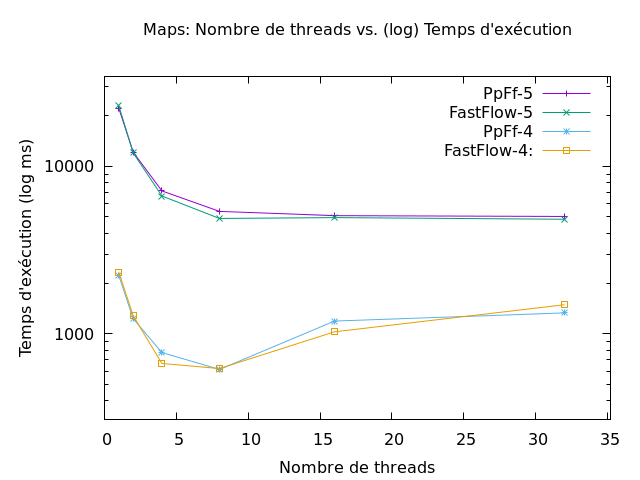
\includegraphics[width=1.0\textwidth]{Figures/graphe_temps_Java_Maps.png}
      \caption{Les temps d'ex\'ecution pour \TT{MicroBenchmarkMaps} sur la machine \M1.}
       \label{GrapheTempsMapsJava.fig}
\end{figure}

\begin{figure}
\centering
     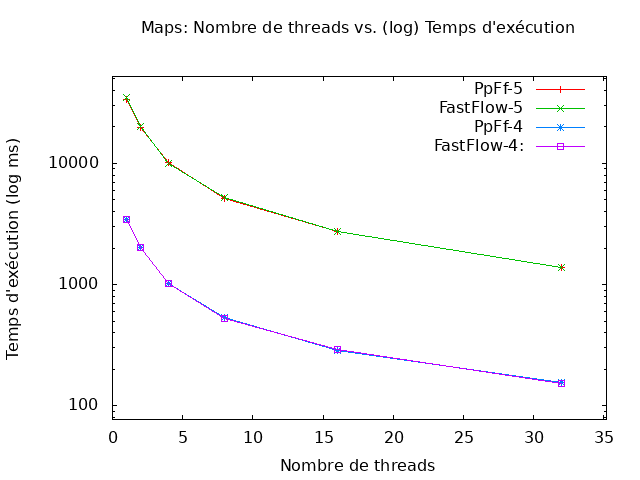
\includegraphics[width=1.0\textwidth]{Figures/graphe_temps_Japet_Maps.png}
      \caption{Les temps d'ex\'ecution pour \TT{MicroBenchmarkMaps} sur la machine \M2.}
       \label{GrapheTempsMapstJapet.fig}
\end{figure}


\gt{Il serait pr\'ef\'erable de pr\'esenter dans l'ordre, tant les figures que la description dans le texte --- \M1\ avant M2.}

La figure~\ref{GrapheTempsMapsJava.fig} montre les r\'esultats des exp\'eriences sur la machine \M1\ alors que la figure~\ref{GrapheTempsMapstJapet.fig} montre les r\'esultats des exp\'eriences sur la machine \M2. On constate un faible surco\^ut
introduit par \TT{PpFf} sur la machine \M1. Ce surco\^ut est plus \'evident lorsque la surcharge du calcul est moins grande. Pourtant, les surco\^uts introduits par \TT{PpFf} par rapport \`a \TT{FastFlow} restent faibles --- c'est ce qui explique, surtout dans la figure~\ref, que les lignes du graph pour \TT{PfFf} et \TT{FastFlow}, tant avec 4 que 5 \emph{threads}, soient quasiment identiques~: la plus grande diff\'erence entre les temps d'ex\'ecutions de deux applications est de presque 300~ms. Le volume de traitement des deux applications est tr\`es grand. Le pipeline est compos\'e de 100~000 \'el\'ements et l'algorithme de calcul appliqu\'e \`a chaque \'el\'ement consiste \`a incr\'ementer une valeur de 0 \`a 10~000 dans le cas avec la granularit\'e 4 et de 0 \`a 100~000 avec la granularit\'e 5. Or, en prenant en consid\'eration ce grand volume de traitement des deux applications, ces 300~ms semblent n\'egligeables.

\GT{Tu parles de grand volume de traitement. Il faudrait expliquer un peu plus pourquoi/comment ce volume est grand = 100~000 \'el\'ements trait\'es dans un pipeline plusieurs fois??}

\IC{J'ai expliqu\'e un petit peu le volume de traitement.}


